\section{Автомат Томпсона}
% descriptive documentation : frame
\begin{frame}{Конструкция автомата Томпсона}\only<2> {\vspace{-5pt}}
    \vspace{-5pt}
    \begin{block}{\bf Алгоритм построения $\Thompson(r)$}
        \only<1-2>{Алгоритм работает рекурсивно, разбивая выражение на составляющие его подвыражения, из которых будет построен НКА с использованием набора правил. Точнее, из регулярного выражения $r$ полученный автомат $A$ с переходной функцией $\delta$ учитывает следующие свойства:}
        \begin{wideitemize}
            \only<1> {
                \item $A$ имеет ровно одно начальное состояние $q_{0}$, которое недоступно ни из какого другого состояния. То есть для любого состояния $q$ и любой буквы $a$ $\delta (q,a)$ не содержит $q_{0}$.
                \item $A$ имеет ровно одно конечное состояние $q_{f}$, которое недоступно ни из какого другого состояния. То есть для любой буквы $a$, $\delta (q_{f},a)=\emptyset$.
                \item Пусть $c$ - число конкатенаций регулярного выражения $r$, а $s$ — количество символов, не считая круглых скобок, то есть $\alter, \star, a, \empt$. Тогда число состояний $A$ равно 2$s - c$ (линейно по размеру $r$).
            } \only<2> {
                \item Число переходов, выходящих из любого состояния, не более двух.
                \item Поскольку НКА из $m$ состояний и не более $e$ переходов из каждого состояния может соответствовать строке длиной $n$ за время $O(emn)$, НКА Томпсона может выполнять сопоставление с образцом за линейное время, предполагая алфавит фиксированного размера.
            }
        \end{wideitemize}
    \end{block}
\end{frame} % descriptive documentation

\begin{frame}{Правила} \only<4> {\vspace{-5pt}}
    \vspace{-5pt}
    \only<1-4>{$N(s)$ и $N(t)$ являются NFA подвыражений $s$ и $t$ соответственно.}
    \only<1> {
        Пустое выражение $\empt$ преобразуется в

        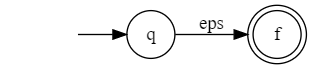
\includegraphics[width=2in, keepaspectratio]{tompson_rule1.png} % the Rule1 diagram placeholder

        Символ $a$ входного алфавита преобразуется в

        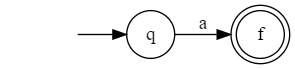
\includegraphics[width=2in, keepaspectratio]{tompson_rule2.png} % the Rule2 diagram placeholder
    }
    \only<2> {
        Выражение объединения $s\alter t$ преобразуется в

        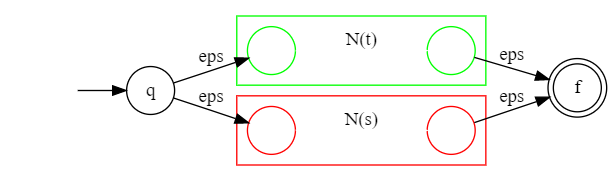
\includegraphics[width=4in, keepaspectratio]{tompson_rule3.png} % the Rule3 diagram placeholder

        Состояние $q$ переходит через $\empt$ либо в начальное состояние $N(s)$, либо $N(t)$. Их конечные состояния становятся промежуточными состояниями всего НКА и сливаются через два $\empt$-перехода в конечное состояние НКА.
    }
    \only<3> {
        Выражение конкатенации $st$ преобразуется в

        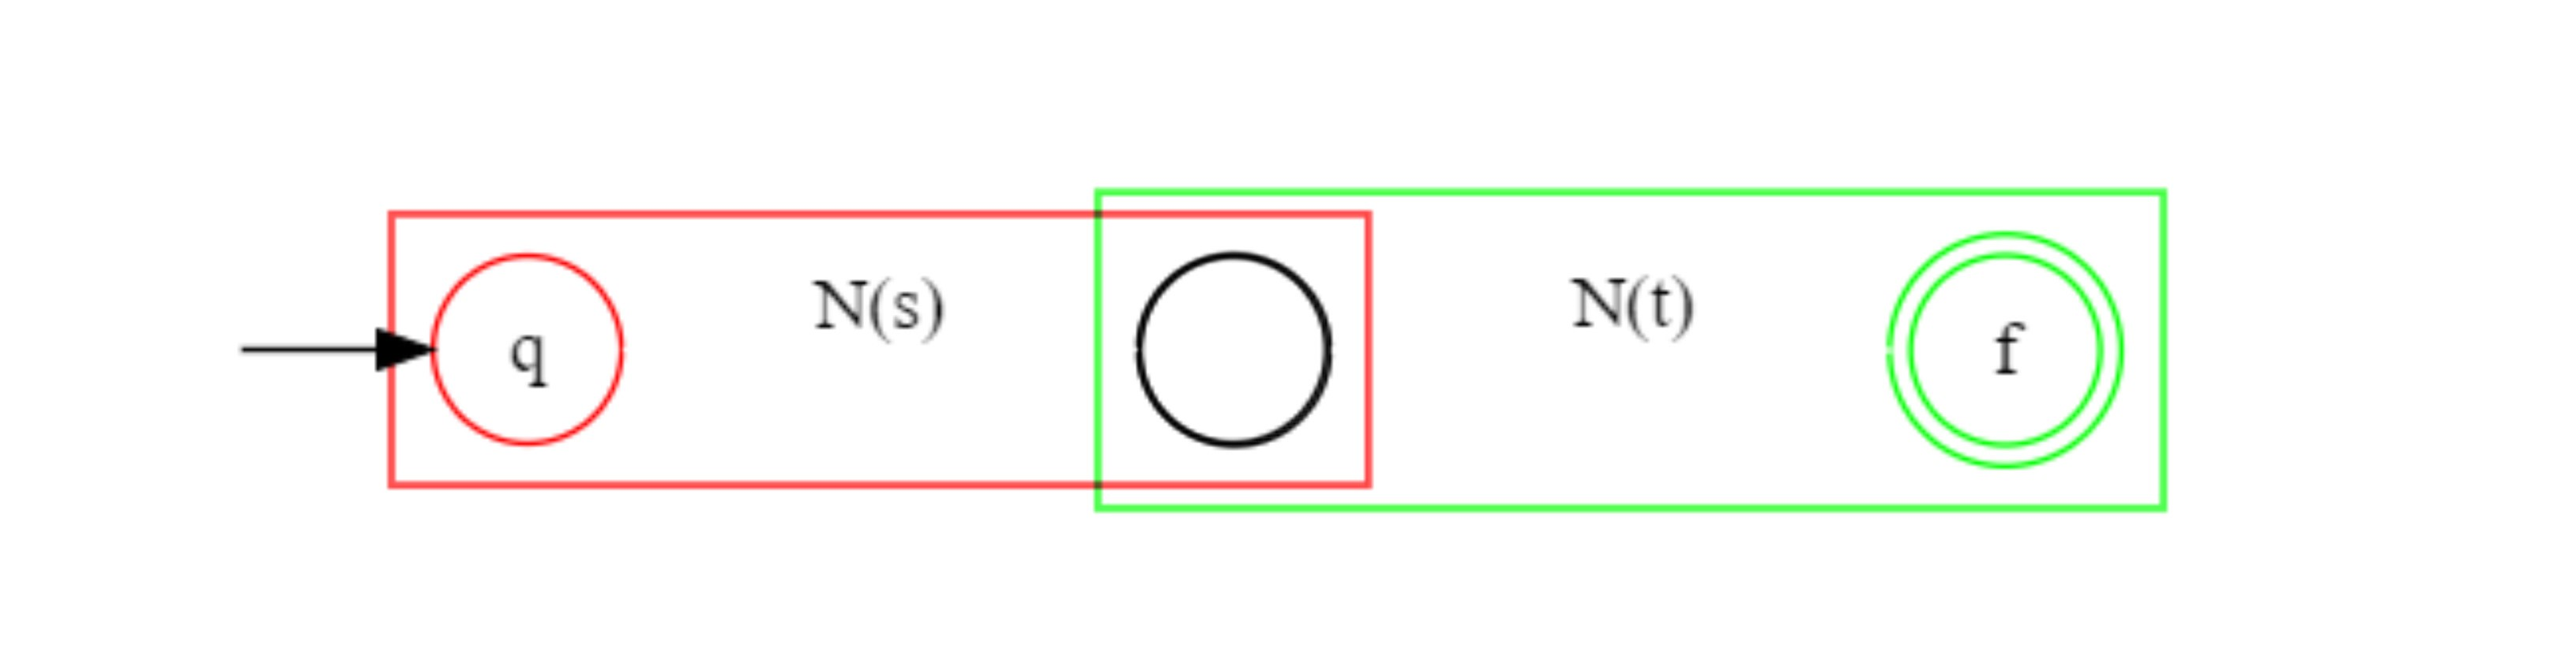
\includegraphics[width=4in, keepaspectratio]{tompson_rule4.png} % the Rule4 diagram placeholder

        Начальное состояние $N(s)$ является начальным состоянием всего НКА. Конечное состояние $N(s)$ становится начальным состоянием $N(t)$. Конечное состояние $N(t)$ является конечным состоянием всего НКА.
    }
    \only<4> {
        Выражение Клини Стар $s\star$ преобразуется в

        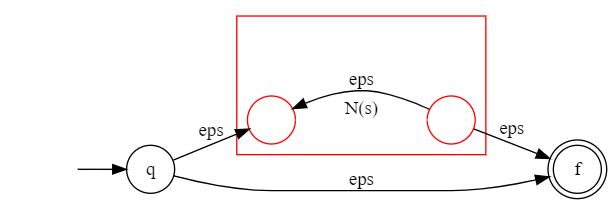
\includegraphics[width=4in, keepaspectratio]{tompson_rule5.png} % the Rule5 diagram placeholder

        $\empt$-переход соединяет начальное и конечное состояние НКА с промежуточным НКА $N(s)$. Другой $\empt$-переход от внутреннего конечного к внутреннему начальному состоянию $N(s)$ допускает повторение выражения $s$ в соответствии с оператором $\star$.

        Заключенное в скобки выражение (выражения) преобразуется в само $N(s)$.
    }
\end{frame}% descriptive documentation

\begin{frame}{Пример автомата Томпсона}
    Исходное регулярное выражение:
    %template_initial_regex % the initial regexp placeholder displaystyle

    Автомат Томпсона:

    %template_thompson % the Thompson diagram placeholder
\end{frame}